\documentclass[t,xcolor={usenames,dvipsnames}]{beamer}

\mode<presentation>
{
\usetheme{Frankfurt}%{Warsaw}
%\setbeamercovered{transparent}
%\setbeamercolor{background canvas}{bg=white}
}

% Delete these, if you do not want the table of contents to pop up at
% the beginning of each (sub)section:
%\AtBeginSubsection[]
%{
%  \begin{frame}<beamer>{Outline}
%    \tableofcontents[currentsection,currentsubsection]
%  \end{frame}
%}
%\AtBeginSection[]
%{
%  \begin{frame}<beamer>{Outline}
%    \tableofcontents[currentsection]
%  \end{frame}
%}

\usepackage[english]{babel}
\usepackage[latin1]{inputenc}
\usepackage{times}
\usepackage[T1]{fontenc}
\usepackage{verbatim}
\usepackage{url}
\usepackage{amsmath,amssymb}
\usepackage{comment}
\usepackage[overlay,absolute]{textpos}
\usepackage{hyperref}

% Author-date citations
\usepackage[authoryear,round]{natbib}
\let\cite=\citep  % default \cite such as {\LaTeX} authors are used to

% Where \includegraphics should look for figures
\graphicspath{{./figs/}{../group_talk_2011_11_29/figs/}}
\usepackage{epstopdf}
\DeclareGraphicsExtensions{.eps,.png,.jpg,.pdf}

% Shortcuts
\newcommand{\myhref}[2]{\href{#1}{\textcolor{Blue}{#2}}}
\newcommand{\myurl}[1]{\myhref{#1}{#1}}
\newcommand{\subitem}[1]{\begin{itemize}[<.->]\item #1 \end{itemize}}
\newcommand{\ghead}[1]{{\tiny #1\\}}
\newcommand{\doi}[1]{\myhref{http://dx.doi.org/#1}{doi:#1}}
\newcommand{\csym}[1]{\textcolor{Blue}{\texttt{#1}}}
\newcommand{\ud}{\mathrm{d}}
\newcommand{\dt}{\ud t}

%%%%%%%%%%%%%%%%%%%%%%%%%%%%%%%%%%%%%%%%%%%%%%%%%%%%%%%%%%%%%%%%%%%%%%
\title{A Brief Introduction To My Interests}
\author{Jonathan Cooper}
\institute[University of Oxford]
{Computational Biology Group\\
 Department of Computer Science\\
 University of Oxford}
\date{April 29, 2014}

\begin{document}

\begin{frame}
\titlepage
\end{frame}


%%%%%%%%%%%%%%%%%%%%%%%%%%%%%%%%%%%%%%%%%%%%%%%%%%%%%%%%%%%%%%%%%%%%%%

%\begin{frame}{Outline}
%\setcounter{tocdepth}{1}
%\tableofcontents
%\end{frame}

%%%%%%%%%%%%%%%%%%%%%%%%%%%%%%%%%%%%%%%%%%%%%%%%%%%%%%%%%%%%%%%%%%%%%%
\section{Functional curation}
\subsection*{Main}
%%%%%%%%%%%%%%%%%%%%%%%%%%%%%%%%%%%%%%%%%%%%%%%%%%%%%%%%%%%%%%%%%%%%%%

\begin{frame}{Using models}
\begin{itemize}
\item As hypothesis encodings, models are developed \emph{for a specific purpose}
  \subitem{May not be appropriate for studying same system in different context}
\item How can we\ldots
  \begin{itemize}
  \item determine a model's functionality, i.e.\ its suitability or limitations for a new study? % Perhaps as part of a composite
  \item re-use a model in a different experimental context?
  \item compare hypotheses: different models' behaviours under the same experiment?
  \end{itemize}
\end{itemize}
\end{frame}


\begin{frame}{Functional curation with virtual experiments}
\subitem{Separate \alert{model structure} and \alert{experimental scenario}}
\vspace{-.2cm}
\hspace{-1cm}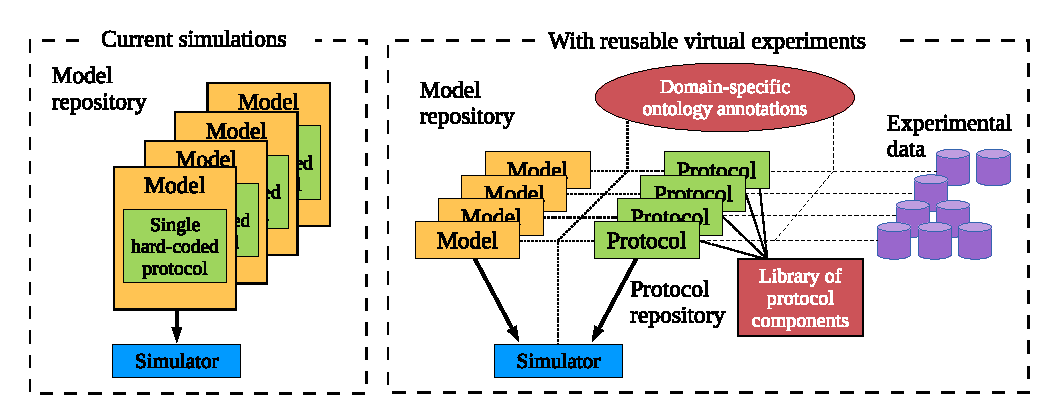
\includegraphics[width=1.185\textwidth]{virtual_expts_schematic}
\vspace{-.31cm}
\begin{itemize}
\item Apply any \alert{virtual experiment} to any (relevant) model
\item One definitive version of each model / protocol
\item Automatically generate post-processed outputs, plots, etc.
\end{itemize}
\end{frame}


\begin{frame}{Exemplar system: Cardiac electrophysiology}
\begin{center}
\vspace{-.5cm}
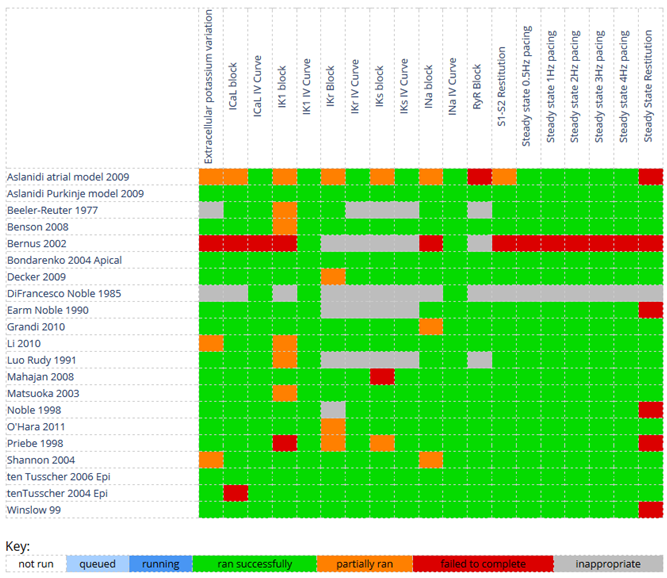
\includegraphics[height=.8\textheight]{cardiac_fc_matrix}\\
\myurl{https://chaste.cs.ox.ac.uk/FunctionalCuration}
\end{center}
\end{frame}


\begin{frame}{Aims}
\begin{itemize}
\item Provide a framework for a coherent approach to model fitting, simulation, comparison and validation
  \begin{itemize}
  \item Continuous evaluation of model predictions against experimental data, throughout model lifecycle
  \item Models that are robust, well tested, and well characterised for particular biological studies
  \end{itemize}
\item A functional curation system \alert{for each domain}
  \begin{itemize}
  \item Brings together competing models, experimental data, and virtual experiments
  \item New models, experiments, or data analysed automatically under all relevant combinations
  \end{itemize}
\end{itemize}
\end{frame}


%%%%%%%%%%%%%%%%%%%%%%%%%%%%%%%%%%%%%%%%%%%%%%%%%%%%%%%%%%%%%%%%%%%%%%
\section{Applications in Ecology}
\subsection*{Main}
%%%%%%%%%%%%%%%%%%%%%%%%%%%%%%%%%%%%%%%%%%%%%%%%%%%%%%%%%%%%%%%%%%%%%%

\begin{frame}{Global ecosystem modelling}
\begin{itemize}
\item `Madingley Model' collaboration with Microsoft Research --- process-based ecosystem modelling
\item Developing a language for describing such models (and experiments)
  \begin{itemize}
  \item Make it easy to change definition of \alert{processes} (e.g.\ predation), \alert{functional groups} (defined by \alert{traits}, e.g.\ feeding mode), etc.
  \item Make it easy to run different experiments
  \end{itemize}
\item Prototype implementation in F\# working, but still very much work in progress \ldots
\end{itemize}
\end{frame}


\begin{frame}{Species distribution modelling}
\begin{center}

\includegraphics[width=\textwidth]{zoon}
\end{center}
\begin{itemize}
\item Held initial discussion workshop in February
\item Interest in creating resource for comparing methods on different (synthetic and real) datasets
  \subitem{Later stage to allow researchers to upload own data for analysis by different methods}
\item Currently pursuing funding and manpower
\end{itemize}
\end{frame}


%%%%%%%%%%%%%%%%%%%%%%%%%%%%%%%%%%%%%%%%%%%%%%%%%%%%%%%%%%%%%%%%%%%%%%
\section{Scientific Software Development}
\subsection*{Main}
%%%%%%%%%%%%%%%%%%%%%%%%%%%%%%%%%%%%%%%%%%%%%%%%%%%%%%%%%%%%%%%%%%%%%%

\begin{frame}{Research software engineering}
\begin{itemize}
\item How should software for science be developed?
\item How can we train researchers to produce `better' software more easily?
  \subitem{The `Software Carpentry' effort}
\item Working with different groups to help in their development efforts
\end{itemize}
\end{frame}


%%%%%%%%%%%%%%%%%%%%%%%%%%%%%%%%%%%%%%%%%%%%%%%%%%%%%%%%%%%%%%%%%%%%%%
\appendix

\begin{frame}{Acknowledgments}
Gary Mirams, Erich Kerekes, Martin Scharm, Aidan Daly\\
Chaste team\\
Alan Garny, Steven Niederer, David Gavaghan

Reference publication: \doi{10.1016/j.pbiomolbio.2011.06.003}\\
Website: \myurl{https://chaste.cs.ox.ac.uk/FunctionalCuration}

\begin{center}

\includegraphics[scale=.9]{chaste-266x60}\\ \vspace{.3cm}

\includegraphics[scale=.7]{logo2020science}\\ \vspace{.4cm}

\includegraphics[width=.55\textwidth]{EPSRC1RGBLO} \hspace{.1cm}

\includegraphics[scale=.55]{logo_msr}
\end{center}
\end{frame}

%%%%%%%%%%%%%%%%%%%%%%%%%%%%%%%%%%%%%%%%%%%%%%%%%%%%%%%%%%%%%%%%%%%%%%

\begin{frame}{What goes in a protocol?}
\begin{itemize}
\item Definition of the interface with the model being experimented on
  \begin{itemize}
  \item Handle variations in modelling conventions: naming, encoding the biology in mathematics
  \item Units conversions
  \item Isolate relevant sub-model(s), using model inputs \& outputs of interest
  \end{itemize}
\item Definition of simulations to perform
\item Post-processing operations on simulation results
\item Description of what to plot
\vspace{.5cm}
\item Also language features facilitating building complex protocols, e.g.\ protocol inputs, outputs, and imports.
\end{itemize}
\end{frame}

\begin{frame}{Our protocol structure}
\begin{center}
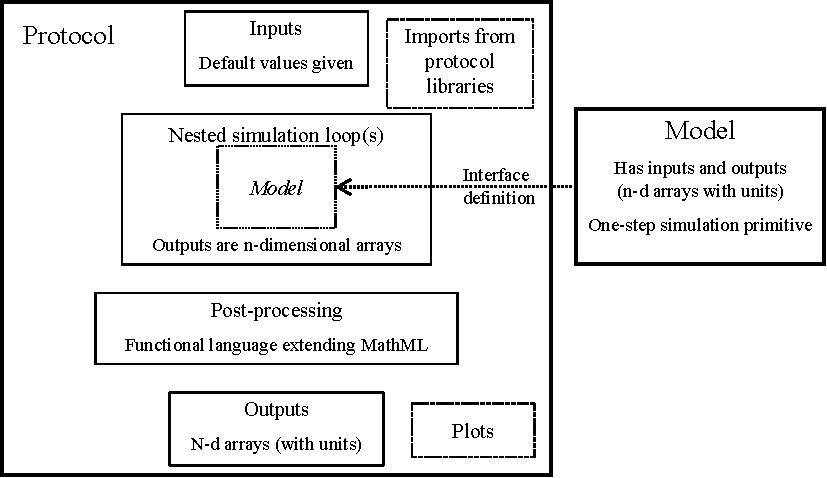
\includegraphics[width=\textwidth]{protocol_language}
\end{center}
\end{frame}

\begin{frame}{Challenges arising from cell-based work}
\begin{itemize}
\item Setting `biological' parameters that don't have direct representations in all models
  \subitem{Or vary spatially}
\item Describing the coupling of component models
\item Cell birth \& death imply non-regular result arrays
  \subitem{Increases technical complexity of post-processing}
\item What post-processing should be in the protocol language?
  \begin{itemize}[<.->]
  \item What is best as dedicated code or workflow?
  \item A language targeted at protocol exchange should be supportable by multiple tools
  \item Contrast: rapid prototyping, or deposition in a repository of standard experiments
  \end{itemize}
\end{itemize}
\end{frame}

\end{document}
